\documentclass[a4paper]{article}

\usepackage[english]{babel}
\usepackage[utf8]{inputenc}
\usepackage{amsmath}
\usepackage{graphicx}
\usepackage[colorinlistoftodos]{todonotes}
\usepackage[left=2cm, right=2cm, top=2cm]{geometry} 
\usepackage{float}
\title{$S_N$ Method}

\author{Amelia Trainer}

\date{\today}

\begin{document}
\maketitle


\section*{Homogenous Slab}
Here are the convergence plots for a 50 cm slab homogeneous slab, using 10,000 cells to be the ``good'' answer with which to judge my errors on.\\
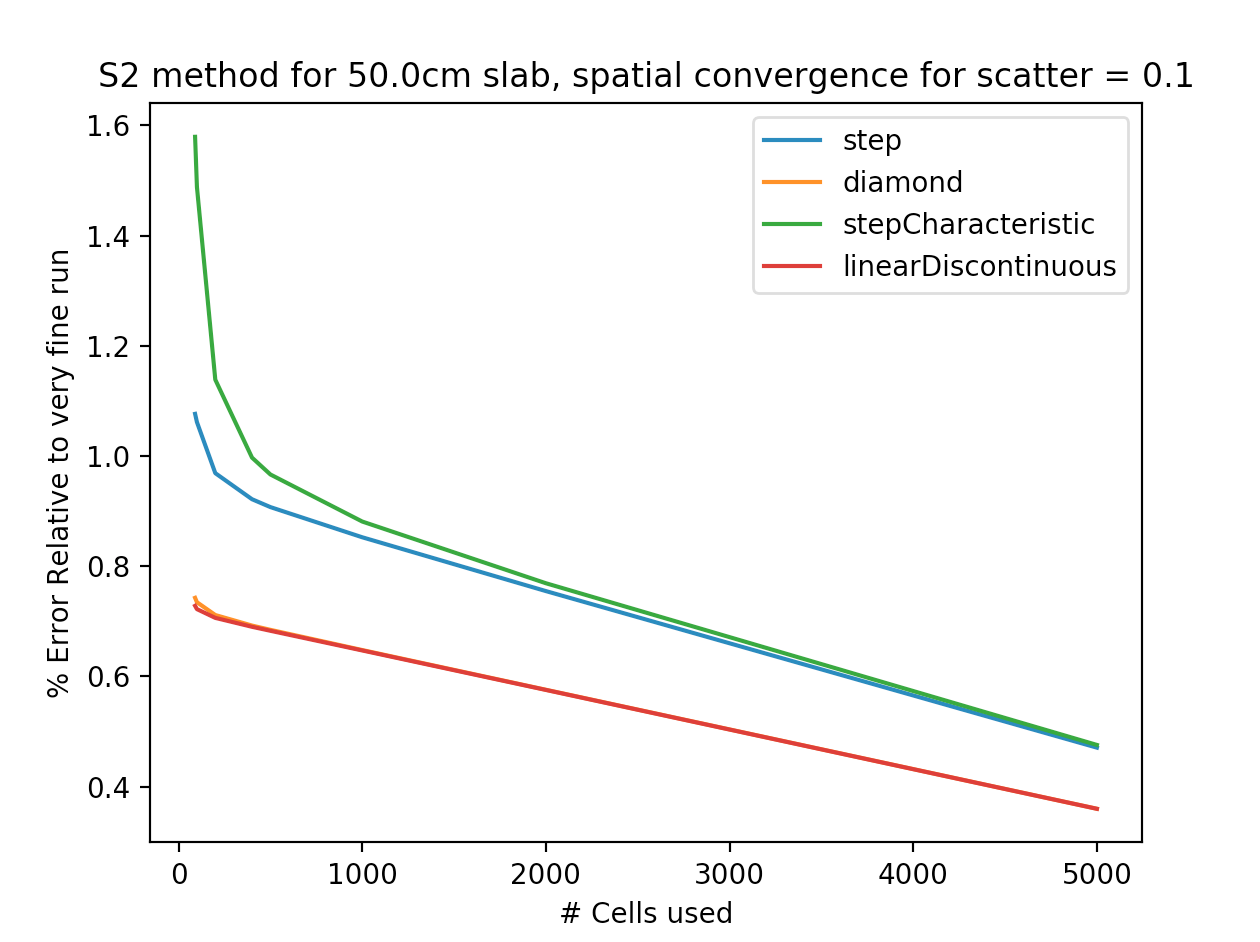
\includegraphics[width=0.5\textwidth]{f2}
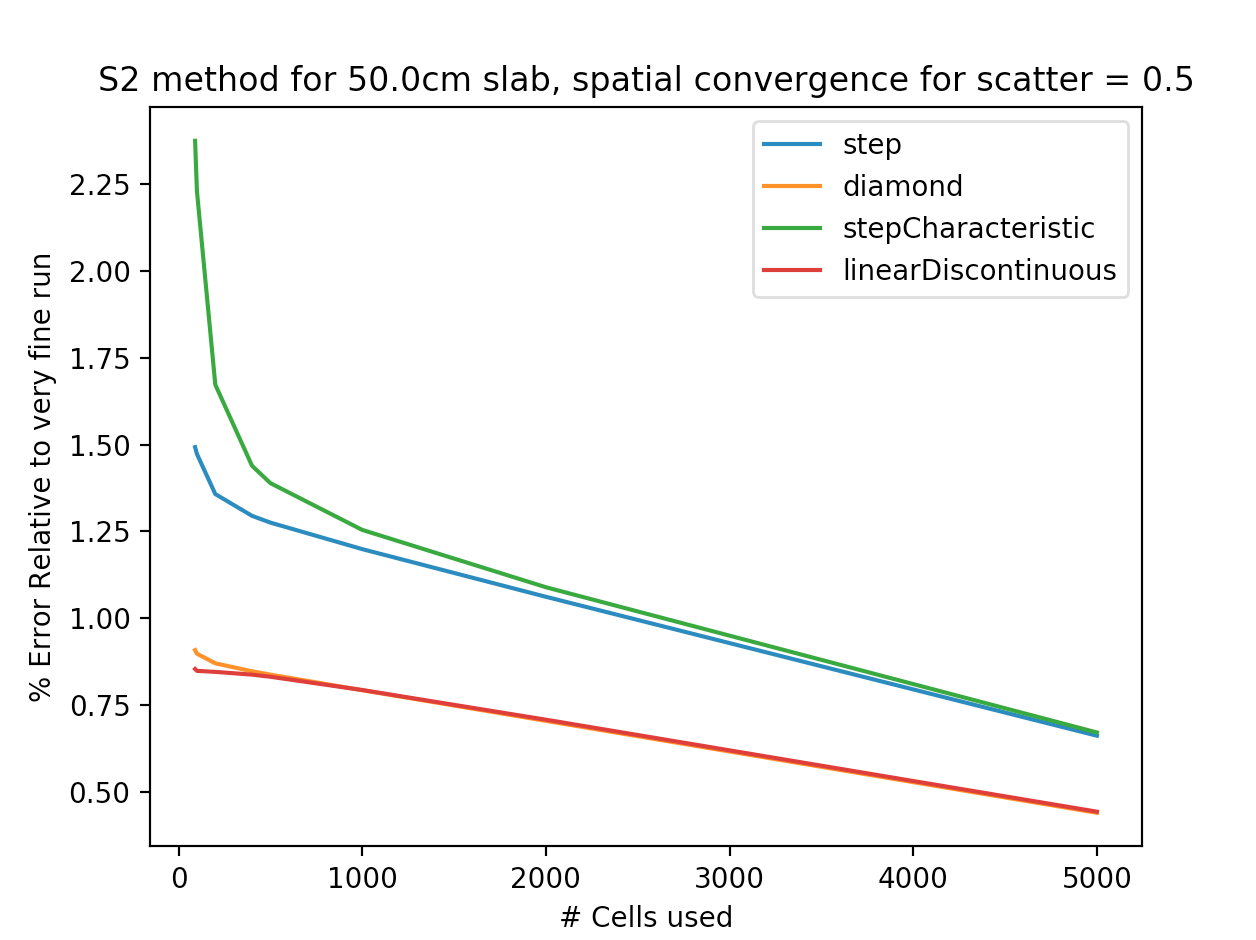
\includegraphics[width=0.5\textwidth]{f3}\\

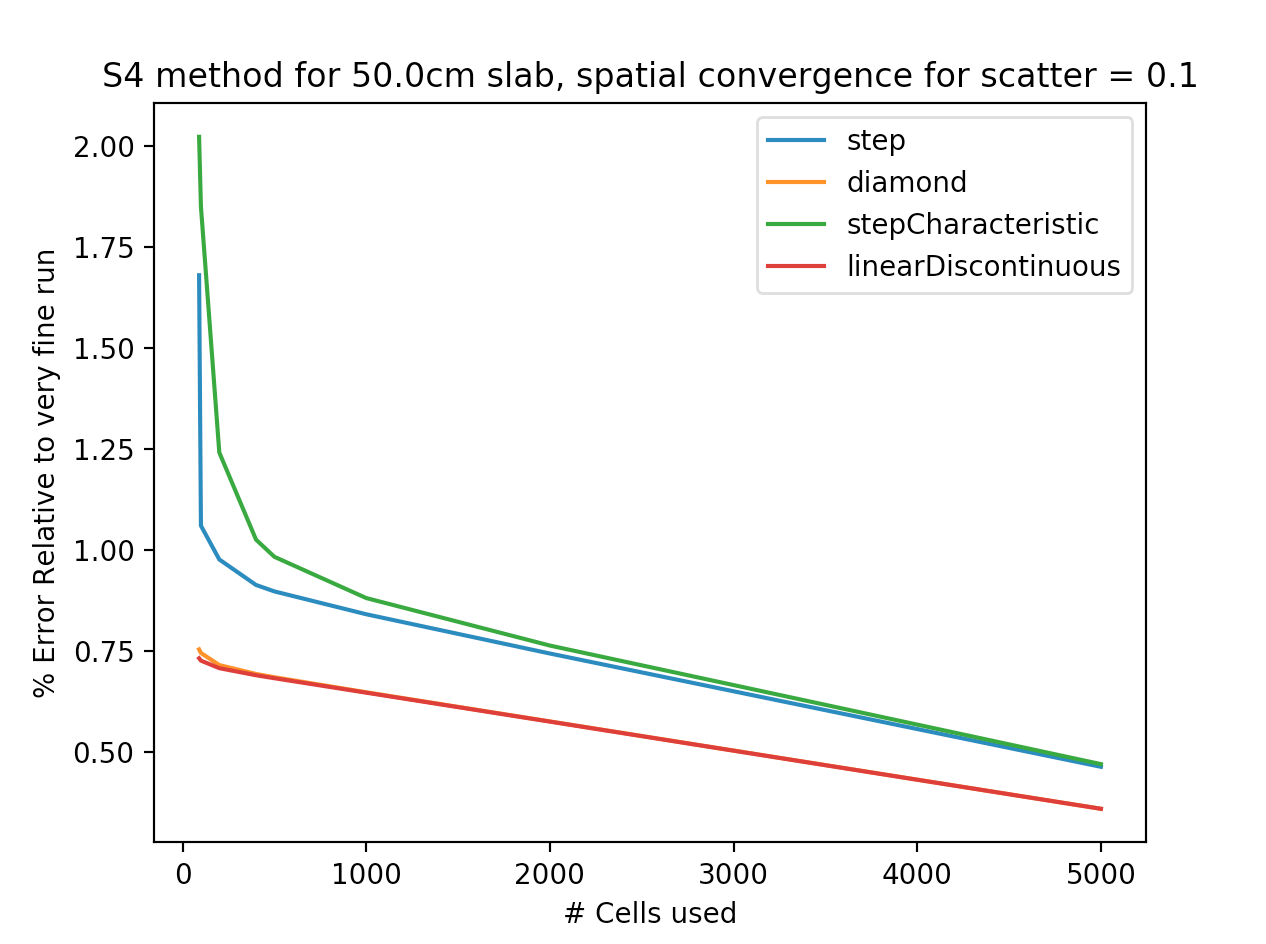
\includegraphics[width=0.5\textwidth]{f1}
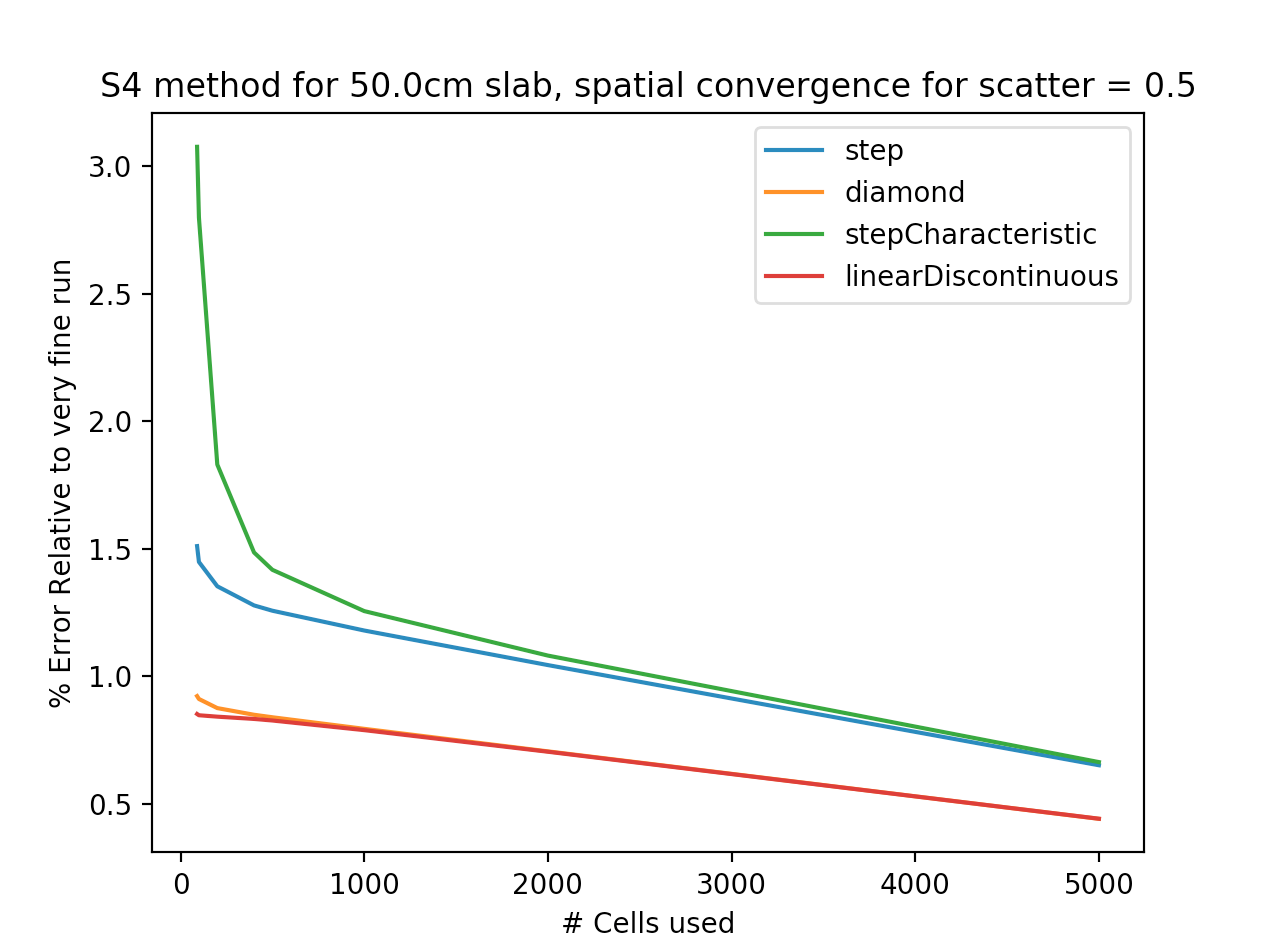
\includegraphics[width=0.5\textwidth]{f4}\\

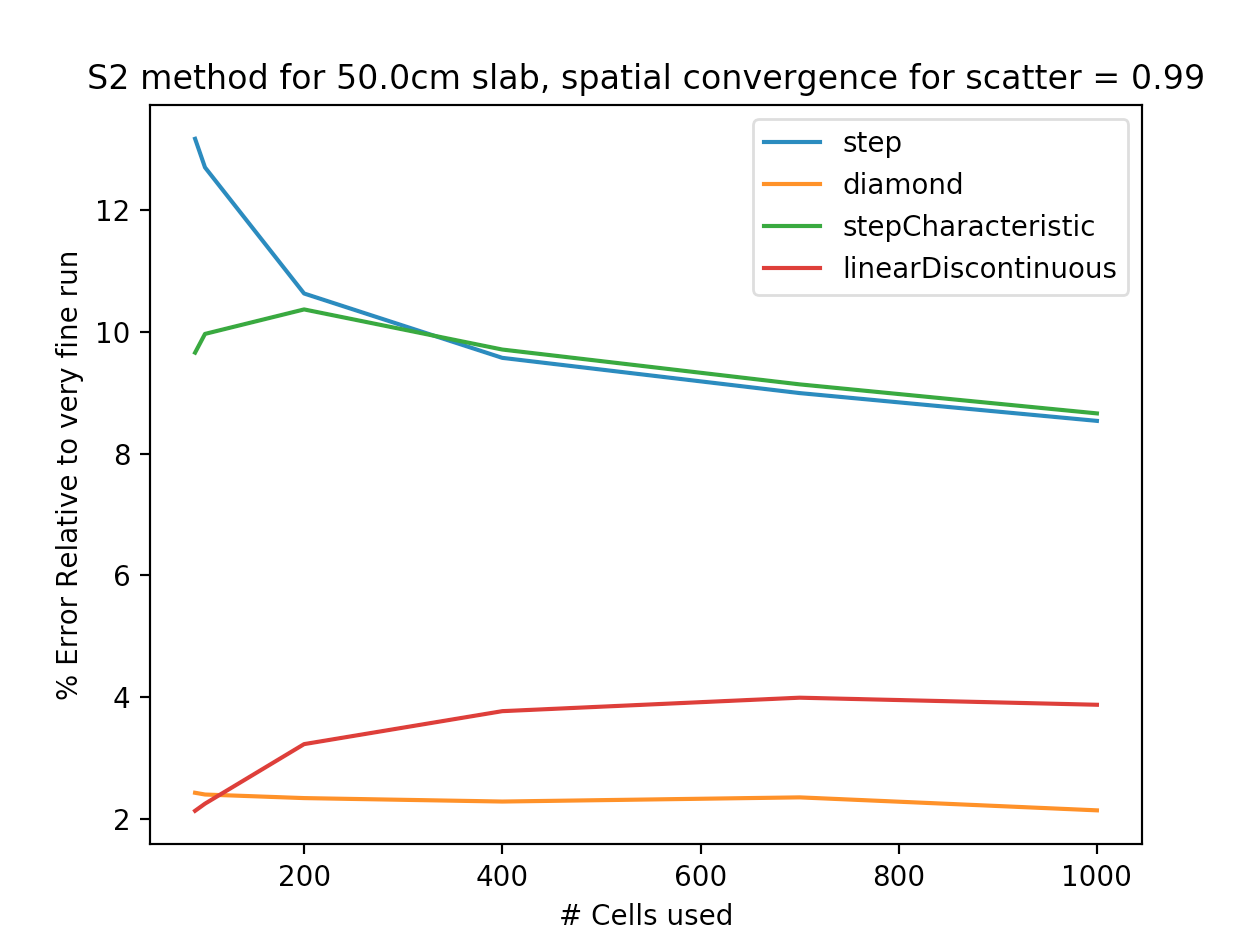
\includegraphics[width=0.5\textwidth]{f6}
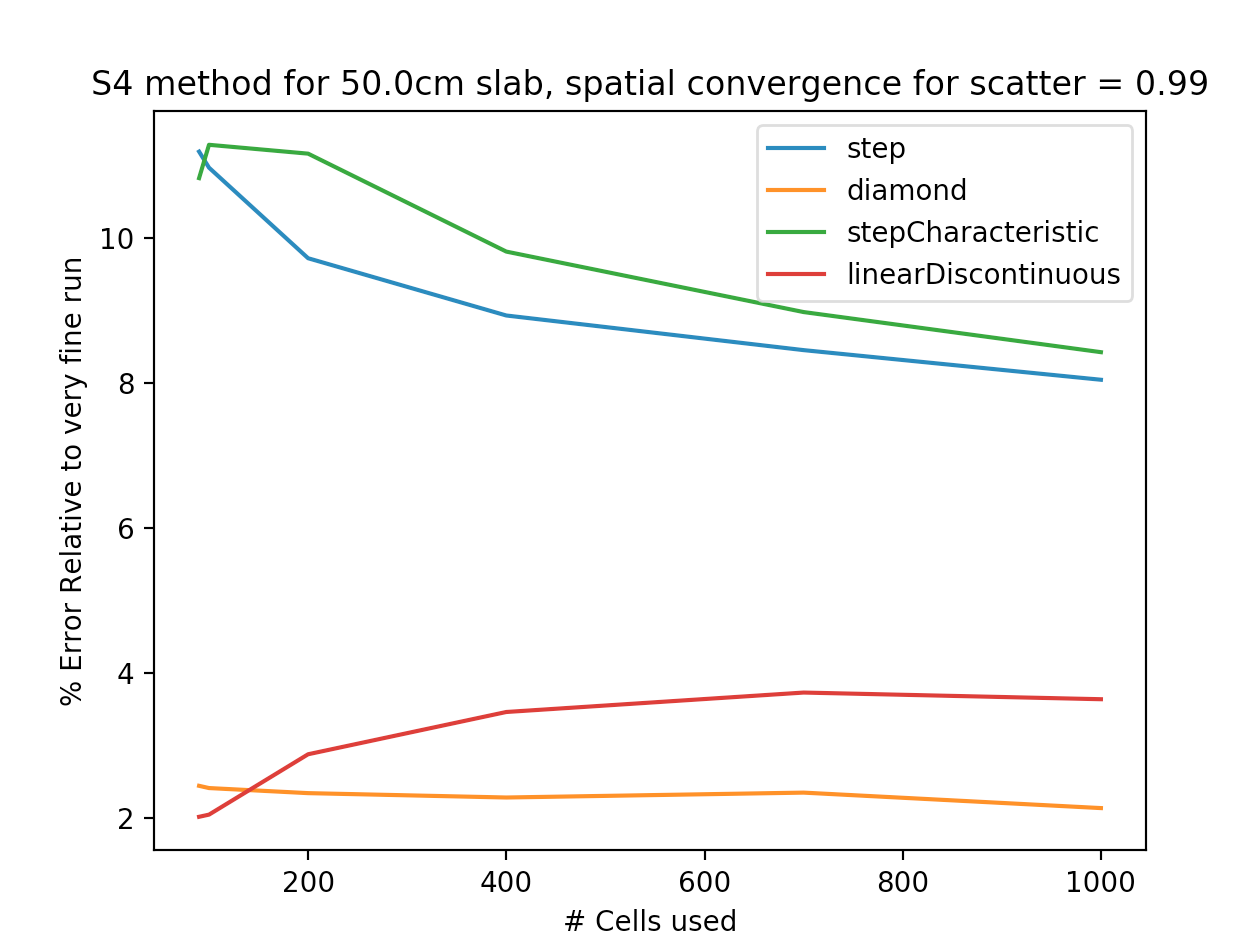
\includegraphics[width=0.5\textwidth]{f5}\\

It seems that for all methods, having a SigS = 0.1 requires 6 iterations, having a SigS = 0.5 requires 18 iterations, and SigS = 0.99 requires about 700-800 iterations (depending on mesh size), except for Step Characteristic which requires as few as 200 iterations for 0.99 SigS value.\par
S2,S4 Step SigS = 0.1  = 6\par
S2,S4 Step SigS = 0.5  = 18\par
S2,S4 Step SigS = 0.99 = 700-800 for various numbers of cells\par~\par

S2,S4 Diamond SigS = 0.1  = 6\par
S2,S4 Diamond SigS = 0.5  = 18\par
S2,S4 Diamond SigS = 0.99 = 700-800 for various numbers of cells\par~\par

S2,S4 Step Characteristic SigS = 0.1  = 6\par
S2,S4 Step Characteristic SigS = 0.5  = 18\par
S2,S4 Step Characteristic SigS = 0.99 = 200-700 for various numbers of cells\par~\par

S2,S4 Linear Disc. SigS = 0.1  = 6\par
S2,S4 Linear Disc. SigS = 0.5  = 18\par
S2,S4 Linear Disc. SigS = 0.99 = 700ish for various numbers of cells\par~\par


Here are some examples of plots I made\\
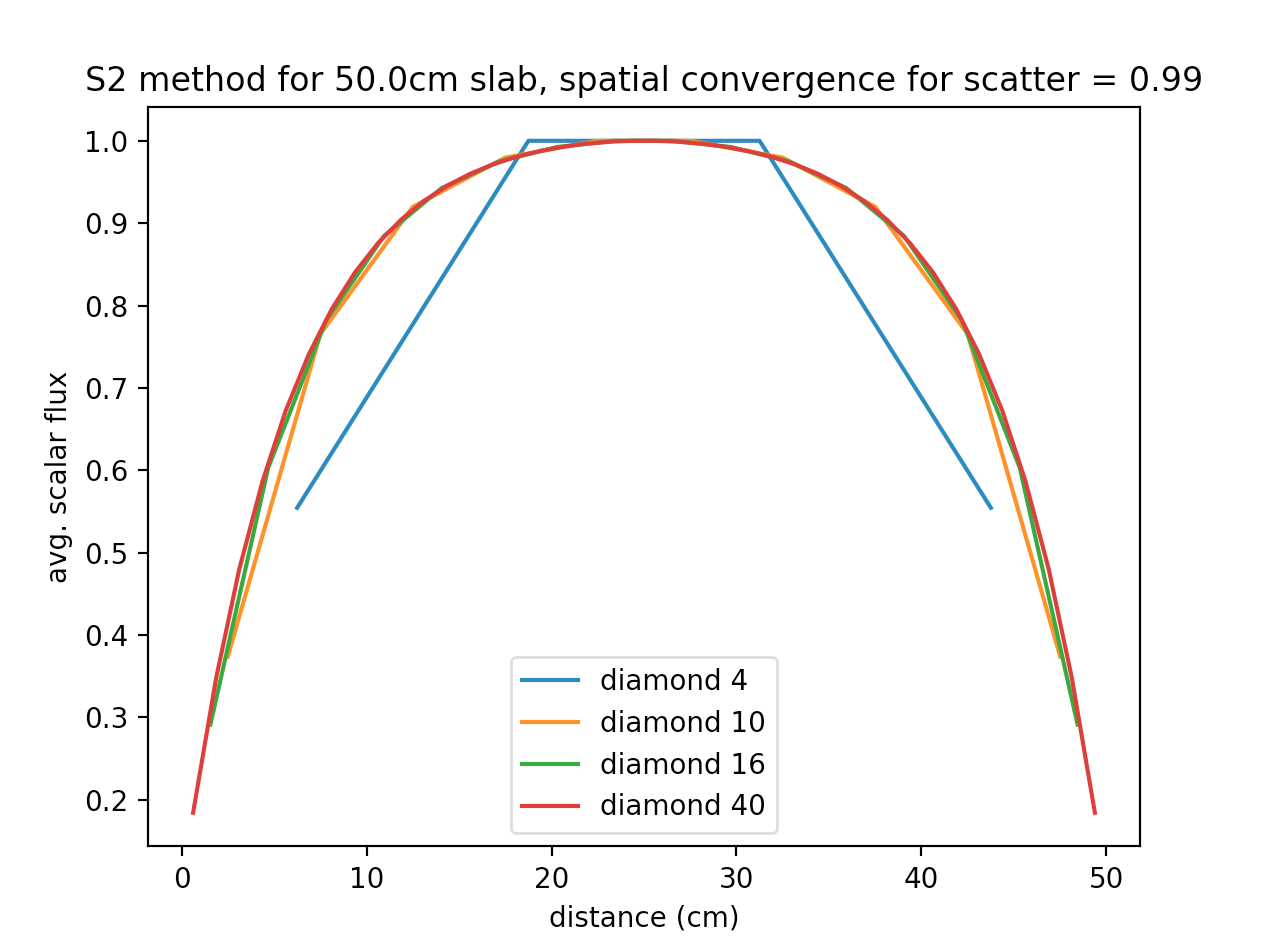
\includegraphics[width=0.5\textwidth]{f8}
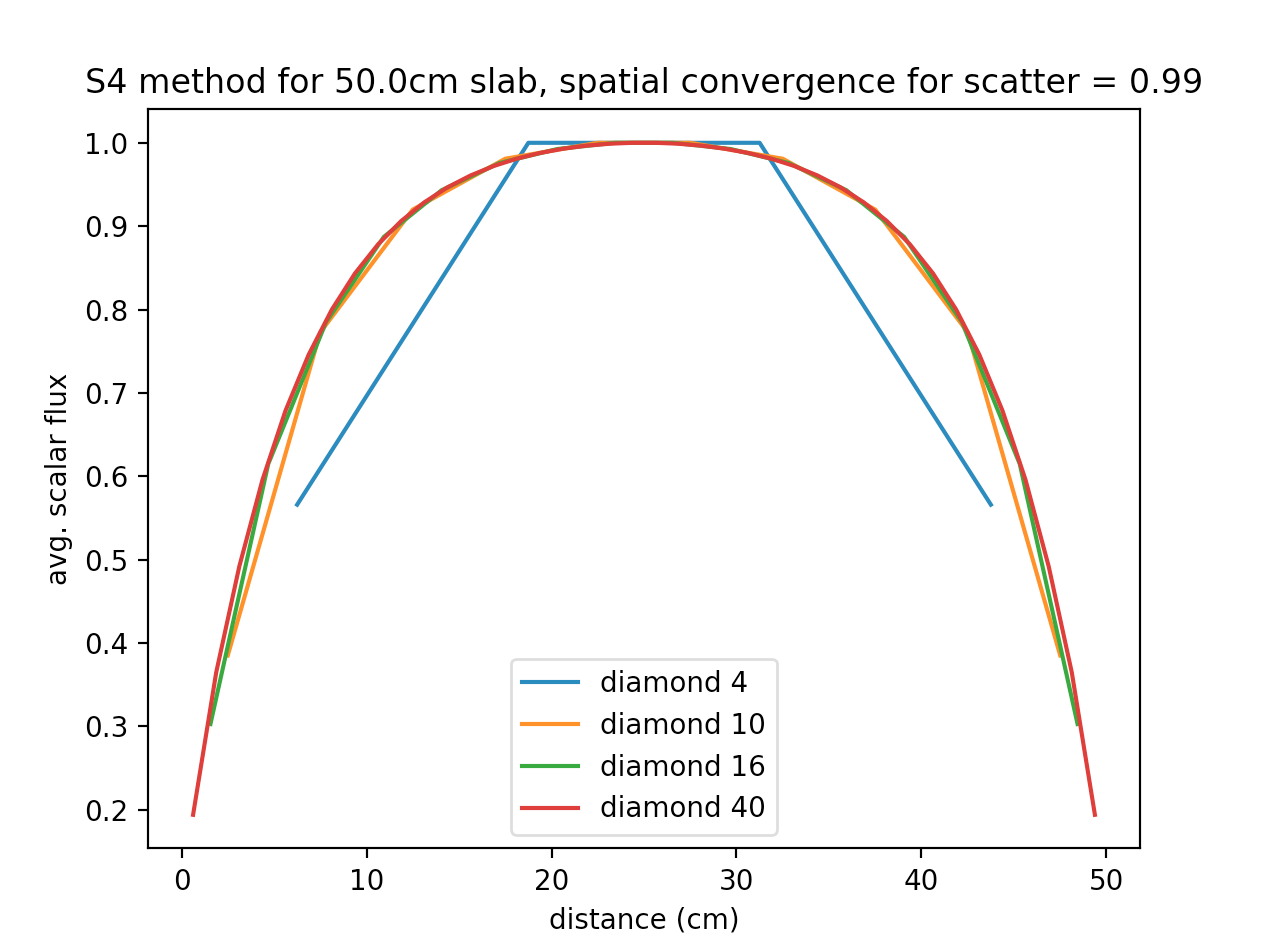
\includegraphics[width=0.5\textwidth]{f9}\\
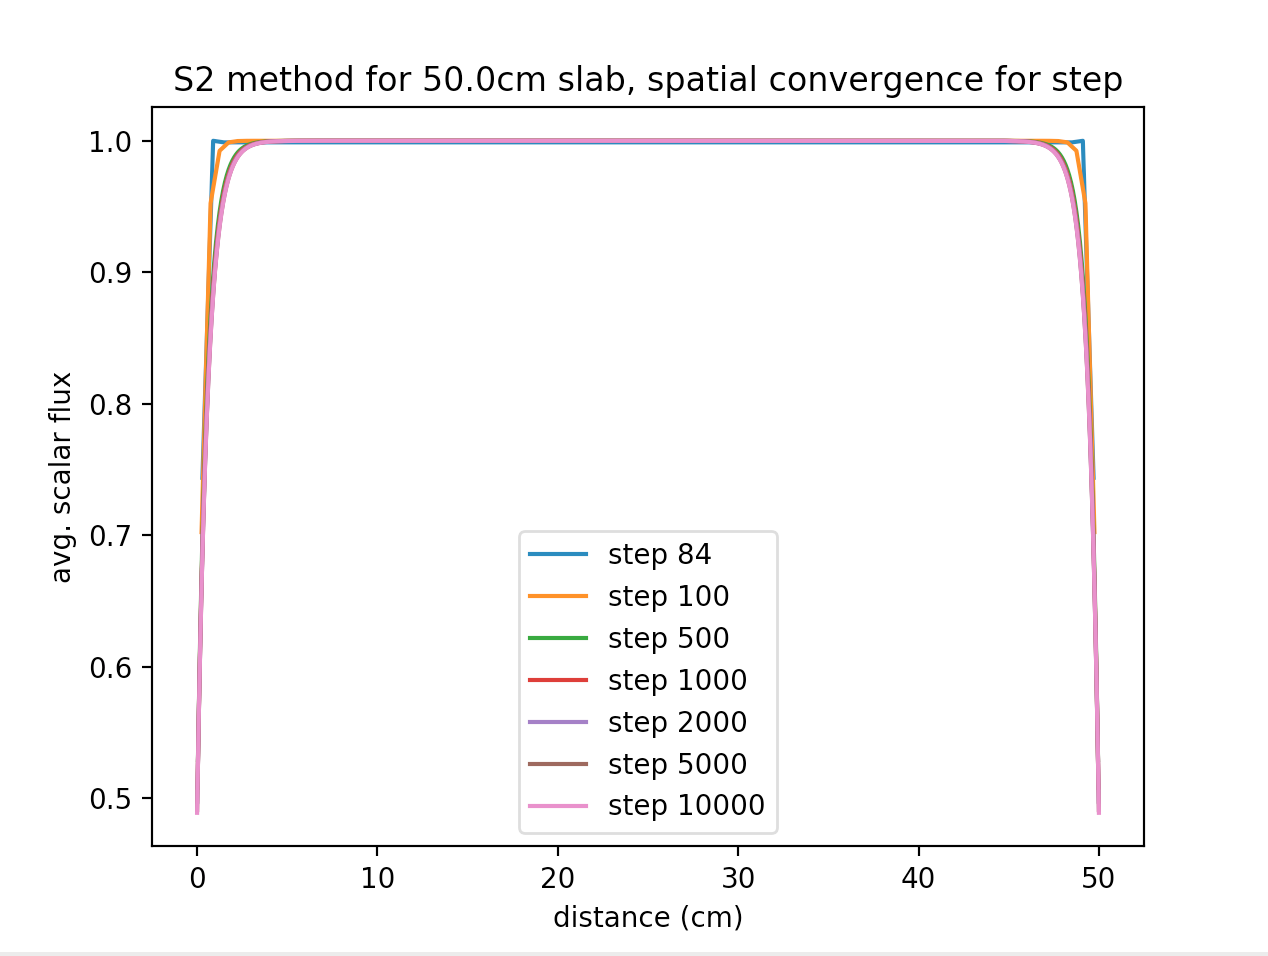
\includegraphics[width=0.5\textwidth]{f10}
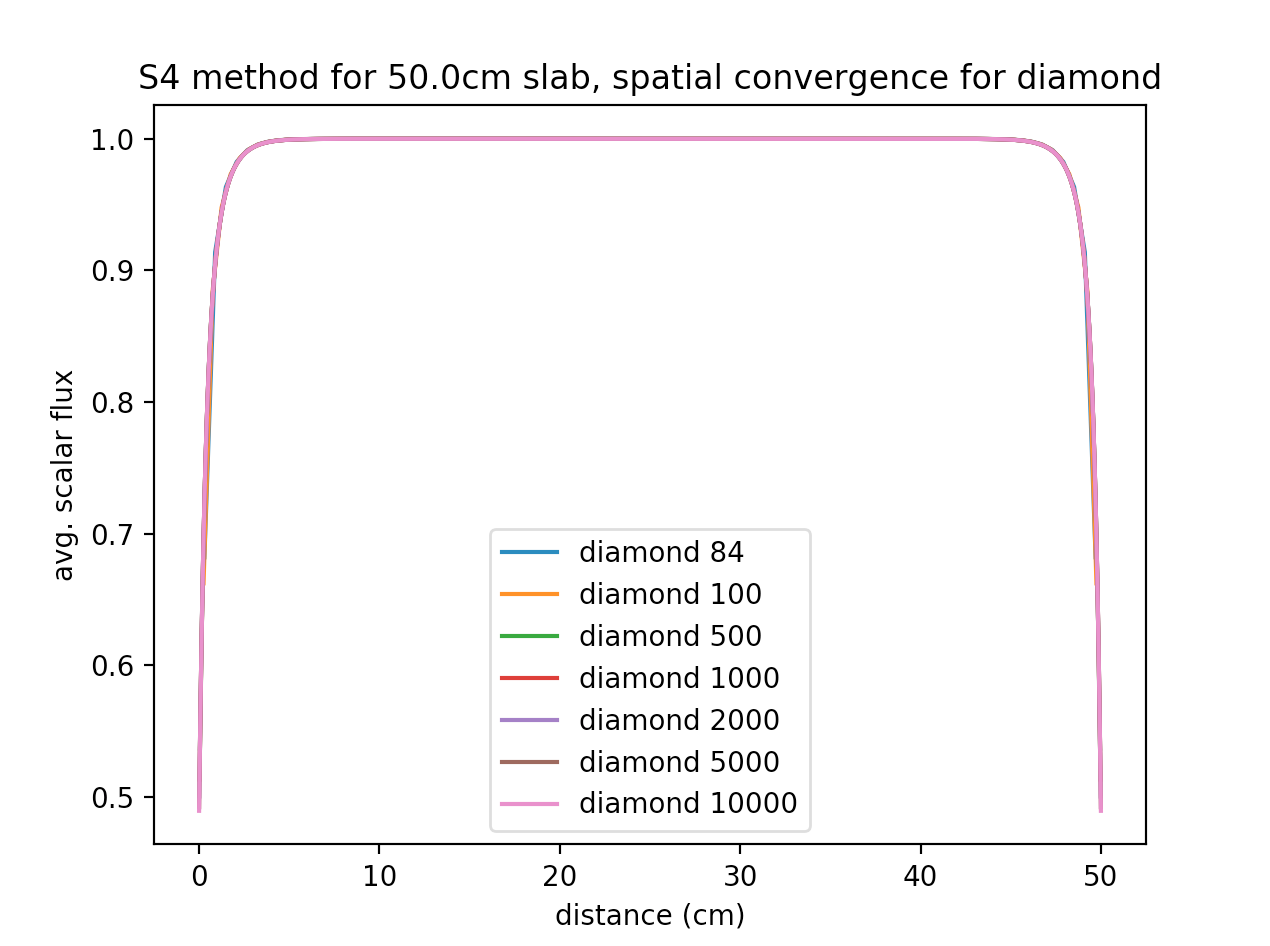
\includegraphics[width=0.5\textwidth]{f11}\\
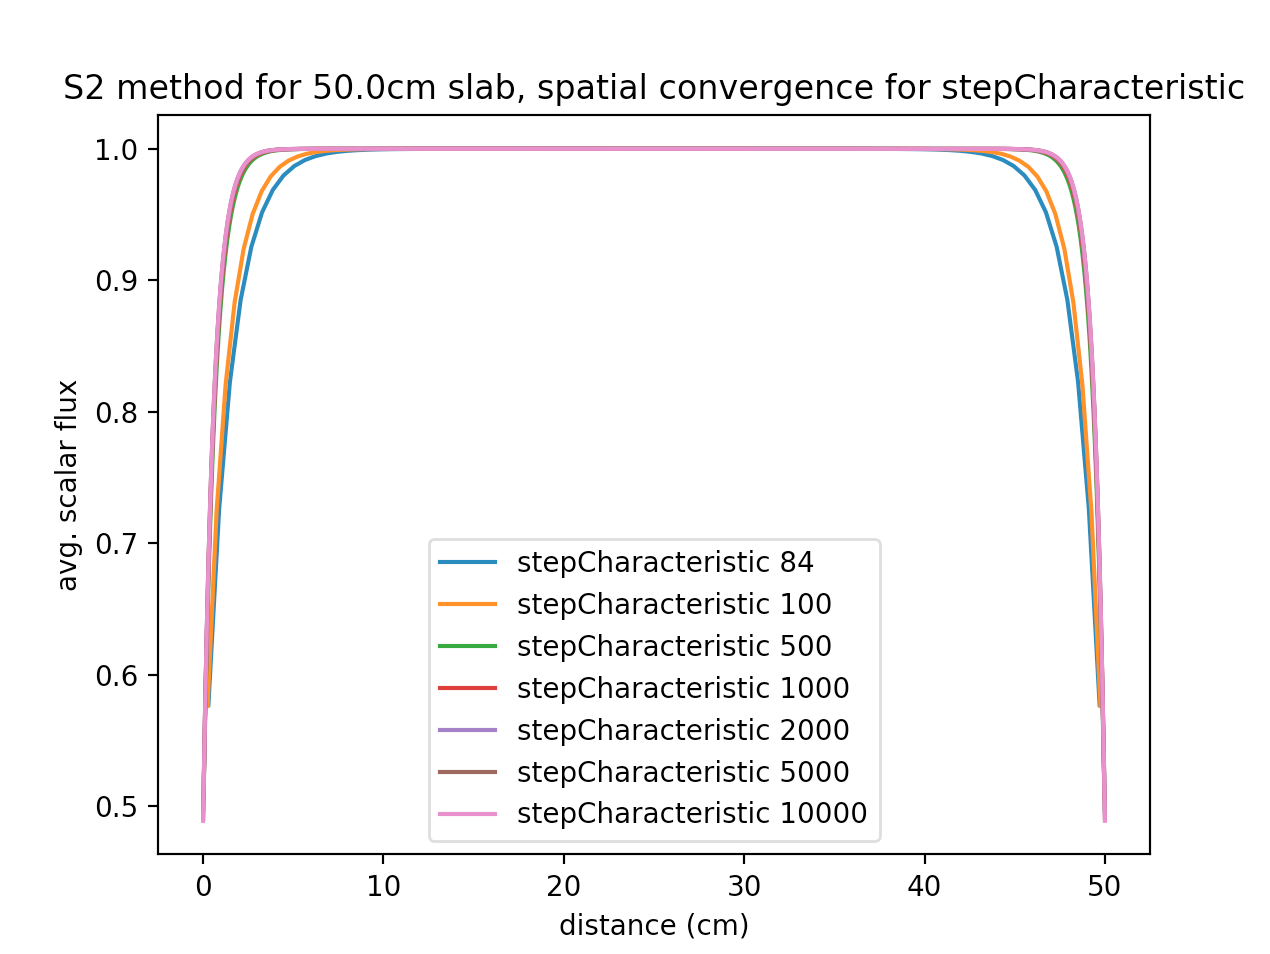
\includegraphics[width=0.5\textwidth]{f12}
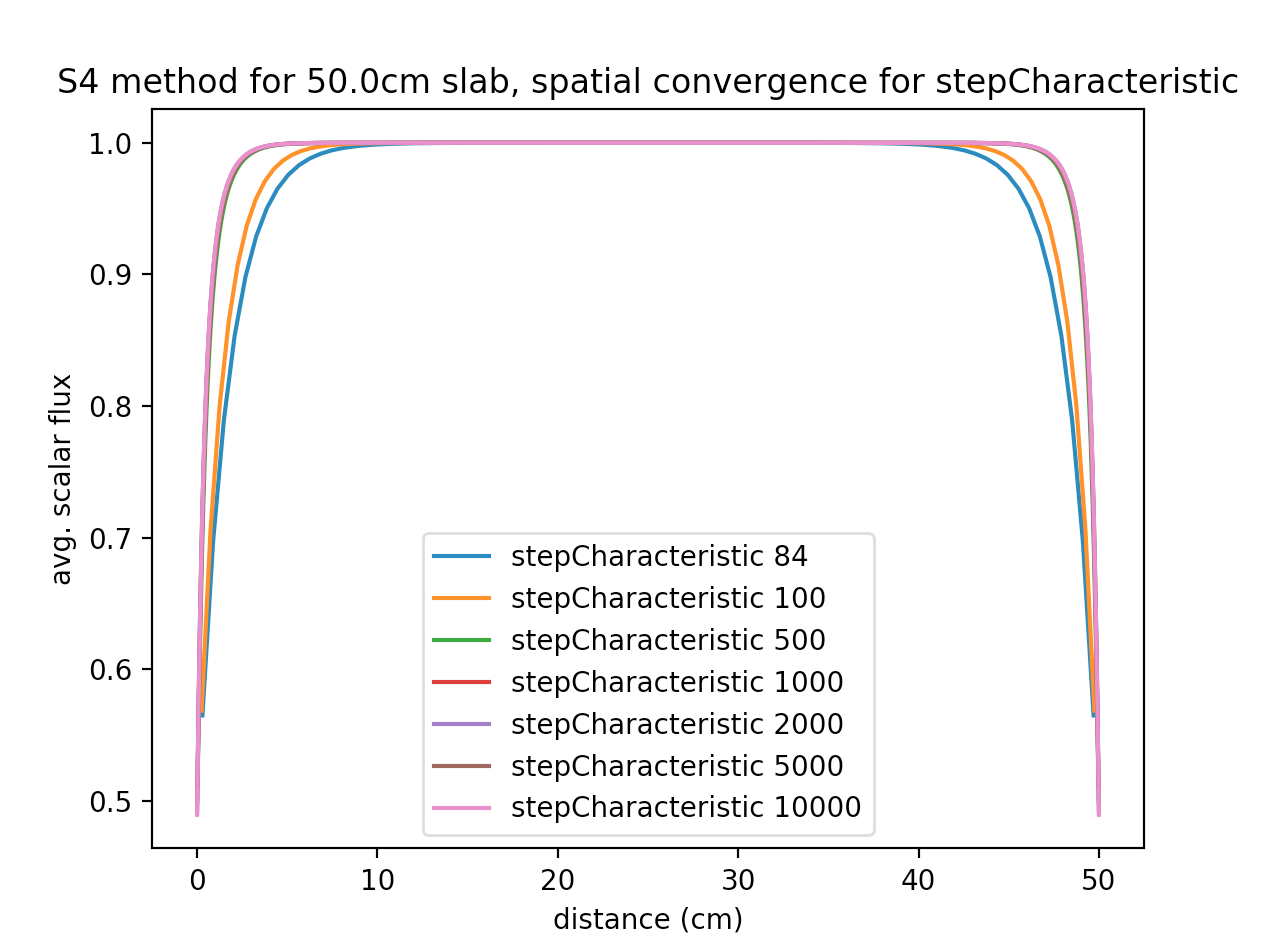
\includegraphics[width=0.5\textwidth]{f13}\\

The number of cells we have is $L/dx$. This means that we will have to store flux in the cell, of which there are $L/dx$, and save the information at the boundaries, of which there are $L/dx + 1$.\par
If we store angular flux in each slab instead of scalar flux, we will have an additional $L/dx\times\#~\mbox{angles}$.\par

\includegraphics[width=0.5\textwidth]{f23}\\





\subsection*{Heterogeneous Slab}
All my methods, for various mesh sizes, took between 15 and 20 iterations to converge.\par
\includegraphics[width=0.5\textwidth]{f17}
\includegraphics[width=0.5\textwidth]{f18}\\
\includegraphics[width=0.5\textwidth]{f19}
\includegraphics[width=0.5\textwidth]{f20}\\
\includegraphics[width=0.5\textwidth]{f21}
\includegraphics[width=0.5\textwidth]{f22}\\








\end{document}
